\documentclass[aspectratio=169]{beamer}
\usepackage[utf8]{inputenc}
\usepackage[T1]{fontenc}
\usepackage[french]{babel}
\usepackage{booktabs}
\usepackage{array}
\usepackage{multirow}
\usepackage{colortbl}
\usepackage{xcolor}
\usepackage{tcolorbox}
\tcbuselibrary{skins,breakable}

% ── THEME ──────────────────────────────────────────────────────────────────
\usetheme{Madrid}
\usecolortheme{default}

\definecolor{bleumed}{RGB}{30,74,140}
\definecolor{bleulair}{RGB}{31,107,142}
\definecolor{vertdoux}{RGB}{39,174,96}
\definecolor{rougealerte}{RGB}{192,57,43}
\definecolor{orangemod}{RGB}{230,126,34}
\definecolor{grisclair}{RGB}{245,245,245}
\definecolor{jaunedoux}{RGB}{255,243,224}
\definecolor{bleupale}{RGB}{235,241,250}
\definecolor{violetdoux}{RGB}{142,68,173}
\definecolor{violetpale}{RGB}{245,235,255}

\setbeamercolor{palette primary}{bg=bleumed, fg=white}
\setbeamercolor{palette secondary}{bg=bleulair, fg=white}
\setbeamercolor{palette tertiary}{bg=bleumed!80, fg=white}
\setbeamercolor{palette quaternary}{bg=bleumed, fg=white}
\setbeamercolor{structure}{fg=bleumed}
\setbeamercolor{section in toc}{fg=bleumed}
\setbeamercolor{frametitle}{bg=bleumed, fg=white}
\setbeamercolor{title}{bg=bleumed, fg=white}
\setbeamercolor{block title}{bg=bleumed, fg=white}
\setbeamercolor{block body}{bg=bleupale}
\setbeamercolor{block title alerted}{bg=rougealerte, fg=white}
\setbeamercolor{block body alerted}{bg=rougealerte!10}
\setbeamercolor{block title example}{bg=vertdoux, fg=white}
\setbeamercolor{block body example}{bg=vertdoux!10}

\setbeamerfont{title}{size=\Large, series=\bfseries}
\setbeamerfont{frametitle}{size=\normalsize, series=\bfseries}
\setbeamertemplate{navigation symbols}{}
\setbeamersize{text margin left=0.4cm, text margin right=0.4cm}

\setbeamertemplate{footline}{
  \leavevmode\hbox{
    \begin{beamercolorbox}[wd=.33\paperwidth,ht=2.25ex,dp=1ex,center]{palette primary}
      \usebeamerfont{author in head/foot}\insertshortauthor
    \end{beamercolorbox}
    \begin{beamercolorbox}[wd=.34\paperwidth,ht=2.25ex,dp=1ex,center]{palette secondary}
      \usebeamerfont{title in head/foot}\insertshorttitle
    \end{beamercolorbox}
    \begin{beamercolorbox}[wd=.33\paperwidth,ht=2.25ex,dp=1ex,right]{palette primary}
      \insertframenumber{} / \inserttotalframenumber\hspace*{2ex}
    \end{beamercolorbox}
  }
}

\newcommand{\oui}{\textcolor{vertdoux}{\textbf{\checkmark}}}
\newcommand{\non}{\textcolor{rougealerte}{\textbf{\texttimes}}}
\newcommand{\partiel}{\textcolor{orangemod}{\textbf{\textasciitilde}}}
\newcommand{\tightlist}{%
  \setlength{\itemsep}{1pt}\setlength{\parskip}{0pt}%
  \setlength{\parsep}{0pt}\setlength{\topsep}{2pt}}

\title[Prédiction complications bariatrique]{%
  Prédiction des complications graves en chirurgie bariatrique\\[4pt]
  \normalsize Scores de comorbidité, modèles statistiques et calculateurs en ligne\\
  \small État de l'art et positionnement de notre étude
}
\author{Izadine M\\ -Sous la supervision du Pr. A LAZZATI}

\date{Mars 2026}

\begin{document}

\begin{frame}[plain]\titlepage\end{frame}
\begin{frame}{Plan}\tableofcontents\end{frame}

% ══════════════════════════════════════════════════════════════════════════
\section{Contexte et rationnel}
% ══════════════════════════════════════════════════════════════════════════

\begin{frame}[shrink=5]{Contexte : la chirurgie bariatrique en France}
  \begin{columns}[T]
    \begin{column}{0.48\textwidth}
      \begin{block}{Rapport IFSO 2024}
        \centering
        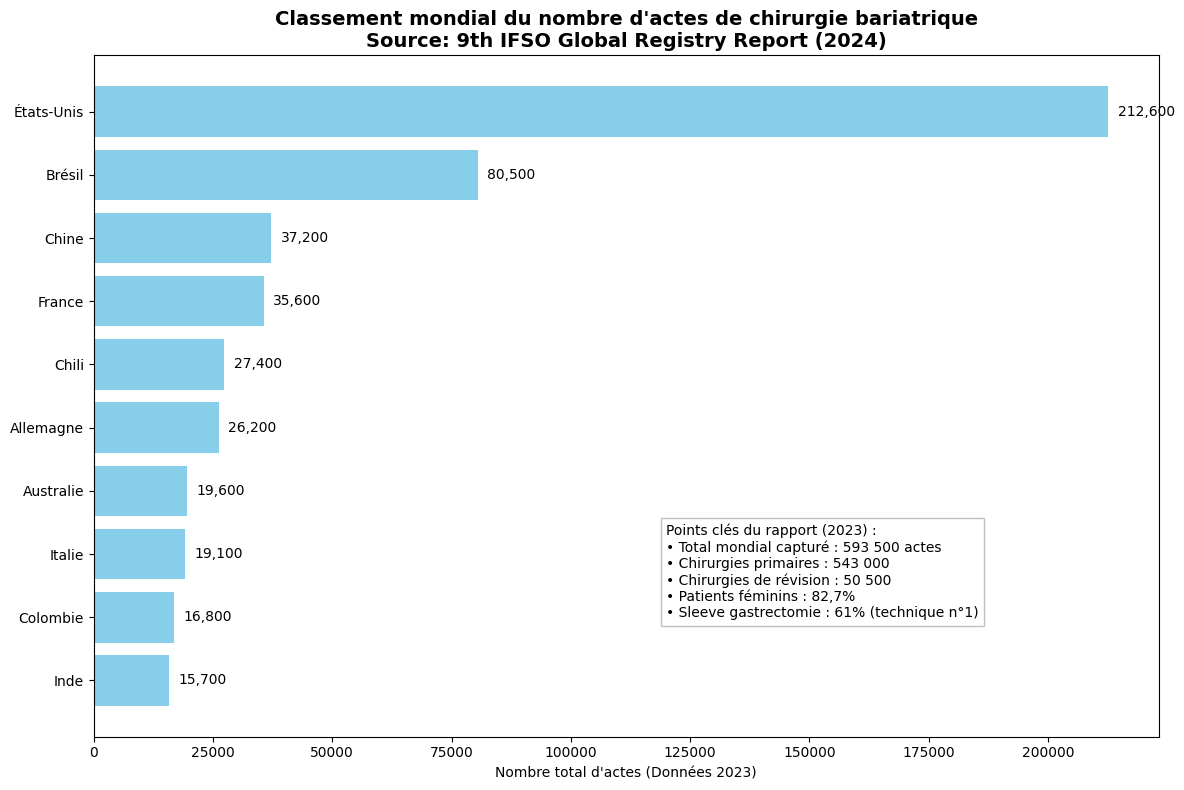
\includegraphics[width=\textwidth]{output.png}
      \end{block}
    \end{column}
    % ... (votre deuxième colonne ici)
    \begin{column}{0.48\textwidth}
      \begin{alertblock}{Le problème central}
        \footnotesize\tightlist
        \begin{itemize}\tightlist
          \item Effets indésirables sévères \textbf{plus fréquents qu'estimé}
          
          \item Comorbidités intégrées de façon \textbf{hétérogène} et non comparée
        \end{itemize}
      \end{alertblock}
    \end{column}
  \end{columns}

\end{frame}

\begin{frame}[shrink=5]{Rationnel : trois stratégies jamais comparées formellement}
  \vspace{-0.3em}
  \begin{columns}[T]
    \begin{column}{0.32\textwidth}
      \begin{tcolorbox}[colback=bleupale,colframe=bleumed,
        title={\small\textbf{Approche 1}},fonttitle=\bfseries\small,top=3pt,bottom=3pt]
        \footnotesize\textbf{Comorbidités individuelles}\\[3pt]
        \begin{itemize}\tightlist
          \item HTA oui/non
          \item DT2 oui/non
          \item SAOS oui/non
          \item Dyslipidémie oui/non
          \item NASH oui/non
        \end{itemize}
        \vspace{3pt}
        \textcolor{orangemod}{\footnotesize Ignore interactions,\\sévérité et contrôle}
      \end{tcolorbox}
    \end{column}
    \begin{column}{0.32\textwidth}
      \begin{tcolorbox}[colback=bleupale,colframe=bleulair,
        title={\small\textbf{Approche 2}},fonttitle=\bfseries\small,top=3pt,bottom=3pt]
        \footnotesize\textbf{Score composite}\\[3pt]
        \begin{itemize}\tightlist
          \item Charlson-Bannay
          \item Score ASA
        \end{itemize}
        \vspace{3pt}
        \textcolor{orangemod}{\footnotesize Jamais validé comme\\prédicteur de Clavien $\geq$3b\\en chirurgie bariatrique}
      \end{tcolorbox}
    \end{column}
    \begin{column}{0.32\textwidth}
      \begin{tcolorbox}[colback=bleupale,colframe=vertdoux,
        title={\small\textbf{Approche 3}},fonttitle=\bfseries\small,top=3pt,bottom=3pt]
        \footnotesize\textbf{Pénalisée (data-driven)}\\[3pt]
        \begin{itemize}\tightlist
          \item LASSO (L1)
          \item Ridge (L2)
          \item Elastic Net
        \end{itemize}
        \vspace{3pt}
        \textcolor{orangemod}{\footnotesize Absente de la littérature\\bariatrique spécifique}
      \end{tcolorbox}
    \end{column}
  \end{columns}
  \vspace{0.3em}
  \begin{alertblock}{\small Lacune majeure}
    \small Aucune étude n'a comparé ces trois stratégies dans une même cohorte sur un outcome Clavien $\geq$3b à \textbf{90 jours}, incluant chirurgies primaires \textbf{et} de révision.
  \end{alertblock}
\end{frame}

% ══════════════════════════════════════════════════════════════════════════
\section{Modèles académiques publiés}
% ══════════════════════════════════════════════════════════════════════════

% ── FINKS 2011 Slide 1 ─────────────────────────────────────────────────
\begin{frame}[shrink=5]{Modèle 1 --- Finks et al. 2011 (MBSC) --- Données \& Variables}
  \begin{columns}[T]
    \begin{column}{0.48\textwidth}
      \begin{block}{Source}
        \footnotesize
        \textbf{Réf. :} Finks JF et al. \textit{Ann Surg} 2011;254(1):10--15\\
        \textbf{Base :} MBSC (Michigan Bariatric Surgery Collaborative)\\
        \textbf{N :} 25~469 \quad \textbf{Période :} 2006--2009
      \end{block}
      \vspace{0.15em}
      \begin{block}{Méthode statistique}
        \footnotesize
        Régression logistique multivariée\\
        + validation interne par \textbf{bootstrap} (1000 itérations)\\
        Sélection par analyse univariée puis multivariée
      \end{block}
      \vspace{0.15em}
      \begin{block}{Outcome prédit}
        \footnotesize
        \textbf{Complication grave à 30 jours} (définition MBSC) :\\
        menace vitale immédiate OU incapacité durable\\
        (fistule avec réopération, TVP/EP, défaillance organe, décès)\\
        \textcolor{rougealerte}{\textit{Pas de Clavien-Dindo}}
      \end{block}
    \end{column}
    \begin{column}{0.48\textwidth}
      \begin{block}{11 variables prédictives}
        \footnotesize
        \begin{tabular}{rl}
          \toprule
          \textbf{N°} & \textbf{Variable} \\
          \midrule
          1 & Âge (continu) \\
          2 & Sexe masculin \\
          3 & IMC préopératoire (continu) \\
          4 & Type de procédure (bypass / anneau / sleeve) \\
          5 & Maladie cardiovasculaire (IDM, insuff. cardiaque) \\
          6 & Maladie pulmonaire (asthme, BPCO) \\
          7 & Insuffisance rénale chronique \\
          8 & Diabète de type 2 préopératoire \\
          9 & Hypertension artérielle \\
          10 & Syndrome d'apnée obstructive du sommeil \\
          11 & Statut fonctionnel (autonomie) \\
          \bottomrule
        \end{tabular}
      \end{block}
    \end{column}
  \end{columns}
\end{frame}

% ── FINKS 2011 Slide 2 ─────────────────────────────────────────────────
\begin{frame}[shrink=5]{Modèle 1 --- Finks et al. 2011 --- Performance \& Limites}
  \begin{columns}[T]
    \begin{column}{0.48\textwidth}
      \begin{block}{Performance}
        \footnotesize
        \begin{tabular}{lc}
          \toprule
          \textbf{Métrique} & \textbf{Valeur} \\
          \midrule
          AUC (c-statistique) & $\approx$ \textcolor{orangemod}{\textbf{0.65}} \\
          Calibration Hosmer-Lemeshow & Acceptable \\
          Validation & Interne (bootstrap) \\
          Validation externe & \textcolor{rougealerte}{\textbf{Absente}} \\
          \bottomrule
        \end{tabular}
      \end{block}
      \vspace{0.2em}
      \begin{exampleblock}{Points forts}
        \footnotesize\tightlist
        \begin{itemize}\tightlist
          \item Premier modèle de prédiction structuré
          \item Grande cohorte multicentrique (n=25~469)
          \item Inclut DT2, HTA, SAOS
          \item Bootstrap 1000 itérations : robuste en interne
        \end{itemize}
      \end{exampleblock}
    \end{column}
    \begin{column}{0.48\textwidth}
      \begin{alertblock}{Limites}
        \footnotesize\tightlist
        \begin{itemize}\tightlist
          \item Validation interne uniquement (bootstrap)
          \item Pas de validation externe indépendante
          \item Pas de Clavien-Dindo : définition ad hoc
          \item Horizon 30 jours : complications différées non captées
          \item Pas de chirurgie de révision incluse
          \item Population mono-État américain (Michigan)
          \item AUC $\approx$0.65 : insuffisante pour stratification individuelle
          \item Pas de score composite (Charlson absent)
          \item NASH absente des variables
          \item Dyslipidémie absente des variables
        \end{itemize}
      \end{alertblock}
    \end{column}
  \end{columns}
\end{frame}

% ── STENBERG 2018 Slide 1 ──────────────────────────────────────────────
\begin{frame}[shrink=5]{Modèle 2 --- Stenberg et al. 2018 (SOReg) --- Données \& Variables}
  \begin{columns}[T]
    \begin{column}{0.48\textwidth}
      \begin{block}{Source}
        \footnotesize
        \textbf{Réf. :} Stenberg E et al. \textit{Obes Surg} 2018;28(7):1869--1875\\
        \textbf{Base :} SOReg (Scandinavian Obesity Surgery Registry)\\
        \textbf{N dév. :} 37~811 \quad \textbf{N val. :} 6~250\\
        \textbf{Période :} 2010--2015
      \end{block}
      \vspace{0.15em}
      \begin{block}{Méthode statistique}
        \footnotesize
        Régression logistique multivariée\\
        Sélection par modélisation pas-à-pas (stepwise)\\
        Validation \textbf{temporelle interne} sur cohorte 2015
      \end{block}
      \vspace{0.15em}
      \begin{block}{Outcome prédit}
        \footnotesize
        \textbf{Clavien-Dindo $\geq$3b à 30 jours} :\\
        intervention sous AG, défaillance organe, décès\\
        \textit{Prévalence : \textbf{3,2\%} de la cohorte}
      \end{block}
    \end{column}
    \begin{column}{0.48\textwidth}
      \begin{block}{14 variables testées}
        \footnotesize
        \begin{tabular}{clc}
          \toprule
          \textbf{N°} & \textbf{Variable} & \textbf{Retenue} \\
          \midrule
          1  & Chirurgie de révision & \oui \\
          2  & Âge & \oui \\
          3  & IMC préopératoire (bas = risque $\uparrow$) & \oui \\
          4  & Tour de taille & \oui \\
          5  & Dyspepsie / GERD & \oui \\
          6  & Année de l'opération & \oui \\
          7  & Sexe & \oui \\
          8  & Score de Charlson (CCI) & \oui \\
          9  & Score ASA & \oui \\
          10 & Hypertension artérielle & \non \\
          11 & Diabète de type 2 & \non \\
          12 & Syndrome d'apnée du sommeil & \non \\
          13 & Dyslipidémie & \non \\
          14 & Type de chirurgie (sleeve vs bypass) & \non \\
          \bottomrule
        \end{tabular}
        \vspace{2pt}
        {\footnotesize\textbf{Prédicteur n°1 :} révision (OR std. 1.19)}
      \end{block}
    \end{column}
  \end{columns}
\end{frame}

% ── STENBERG 2018 Slide 2 ──────────────────────────────────────────────
\begin{frame}[shrink=5]{Modèle 2 --- Stenberg et al. 2018 --- Performance \& Limites}
  \begin{columns}[T]
    \begin{column}{0.48\textwidth}
      \begin{alertblock}{Performance --- Résultats très décevants}
        \footnotesize
        \begin{tabular}{lc}
          \toprule
          \textbf{Métrique} & \textbf{Valeur} \\
          \midrule
          AUC sur données test & \textcolor{rougealerte}{\textbf{0.53}} \\
          Sensibilité & \textcolor{rougealerte}{\textbf{$<$ 1\%}} \\
          Spécificité & $\approx$ 99\% \\
          \bottomrule
        \end{tabular}
        \vspace{4pt}\\
        $\Rightarrow$ Le modèle \textbf{ne détecte pratiquement aucun} patient à risque\\
        $\Rightarrow$ AUC à peine supérieure au hasard
      \end{alertblock}
      \vspace{0.2em}
      \begin{block}{Interprétation des auteurs}
        \footnotesize
        Les variables SOReg sont insuffisantes pour une discrimination individuelle. La richesse des variables disponibles, non la méthode, est le facteur limitant.
      \end{block}
    \end{column}
    \begin{column}{0.48\textwidth}
      \begin{alertblock}{Limites}
        \footnotesize\tightlist
        \begin{itemize}\tightlist
          \item AUC quasi-nulle sur données test (0.53)
          \item Sensibilité $<$1\% : inutilisable individuellement
          \item HTA, DT2, SAOS non retenus comme prédicteurs indépendants
          \item Score de Charlson retenu mais insuffisant seul
          \item Pas de validation externe indépendante
          \item Variables SOReg limitées (pas HbA1c, nutrition, fragilité)
          \item Horizon 30 jours uniquement
          \item Révision présente comme covariable, pas en sous-groupe dédié
          \item NASH absente
          \item Pas d'approche pénalisée testée
        \end{itemize}
      \end{alertblock}
    \end{column}
  \end{columns}
\end{frame}

% ── CAO 2019 Slide 1/2 ────────────────────────────────────────────────
\begin{frame}[shrink=5]{Modèle 3 --- Cao et al. 2019 (SOReg + 29 algo. ML) --- Source \& Algorithmes}
  \begin{columns}[T]
    \begin{column}{0.50\textwidth}
      \begin{block}{Source}
        \footnotesize
        \textbf{Réf. :} Cao Y et al. \textit{J Clin Med} 2019;8(5):668\\
        \textbf{Base :} SOReg \quad \textbf{N :} 44~061\\
        \textbf{Split :} Entraîn. 2010--2014 (37~811) / Test 2015 (6~250)
      \end{block}
      \vspace{0.15em}
      \begin{alertblock}{Performance --- Surajustement massif}
        \footnotesize
        \begin{tabular}{lcc}
          \toprule
          \textbf{Modèle} & \textbf{AUC entr.} & \textbf{AUC test} \\
          \midrule
          Random Forest & $>$0.90 & \textcolor{rougealerte}{\textbf{0.57}} \\
          GBM           & $>$0.90 & \textcolor{rougealerte}{\textbf{0.56}} \\
          LASSO         & $\approx$0.70 & \textcolor{rougealerte}{\textbf{0.53}} \\
          \midrule
          \textbf{Global} & $>$\textbf{0.90} & \textbf{0.50--0.58} \\
          \bottomrule
        \end{tabular}
        \vspace{3pt}\\
        $\Rightarrow$ Le problème est dans les \textbf{données}, pas la méthode
      \end{alertblock}
    \end{column}
    \begin{column}{0.47\textwidth}
      \begin{block}{Ensemblistes}
        \footnotesize\tightlist
        \begin{itemize}\tightlist
          \item Random Forest, GBM, AdaBoost, Bagging, ExtraTrees
        \end{itemize}
      \end{block}
      \vspace{0.1em}
      \begin{block}{Linéaires / régularisés}
        \footnotesize\tightlist
        \begin{itemize}\tightlist
          \item Régression logistique standard
          \item LASSO (L1), Ridge (L2), Elastic Net (L1+L2)
        \end{itemize}
      \end{block}
      \vspace{0.1em}
      \begin{block}{Autres (21 algorithmes)}
        \footnotesize\tightlist
        \begin{itemize}\tightlist
          \item SVM (noyaux linéaire, RBF, polynomial)
          \item K-Nearest Neighbors, Naïve Bayes
          \item CART, LDA, QDA
          \item SGD, MLP, Gaussian Process, Bayesian Ridge
        \end{itemize}
      \end{block}
      \vspace{0.1em}
      \begin{block}{Gestion du déséquilibre}
        \footnotesize SMOTE (Synthetic Minority Over-sampling Technique)
      \end{block}
    \end{column}
  \end{columns}
\end{frame}

% ── CAO 2019 Slide 2/2 ────────────────────────────────────────────────
\begin{frame}[shrink=5]{Modèle 3 --- Cao et al. 2019 --- Variables (14, identiques à Stenberg)}
  \begin{columns}[T]
    \begin{column}{0.55\textwidth}
      \begin{block}{14 variables testées}
        \footnotesize
        \begin{tabular}{rl}
          \toprule
          \textbf{N°} & \textbf{Variable} \\
          \midrule
          1  & Chirurgie de révision (oui/non) \\
          2  & Âge \\
          3  & IMC préopératoire \\
          4  & Sexe \\
          5  & Score ASA (I à IV) \\
          6  & Score de Charlson (CCI) \\
          7  & Tour de taille \\
          8  & Dyspepsie / GERD (oui/non) \\
          9  & Hypertension artérielle (oui/non) \\
          10 & Diabète de type 2 (oui/non) \\
          11 & Syndrome d'apnée du sommeil (oui/non) \\
          12 & Dyslipidémie (oui/non) \\
          13 & Année de l'opération \\
          14 & Type de chirurgie (sleeve / bypass) \\
          \bottomrule
        \end{tabular}
      \end{block}
    \end{column}
    \begin{column}{0.42\textwidth}
      \begin{alertblock}{Conclusion générale}
        \footnotesize\tightlist
        \begin{itemize}\tightlist
          \item 29 algorithmes testés, dont les plus puissants (RF, GBM, XGB)
          \item Toutes les AUC sur données test : \textbf{0.50--0.58}
          \item Surajustement massif (AUC entraîn. $>$0.90)
          \item SMOTE n'améliore pas la généralisation
          \item La limite est dans les \textbf{variables disponibles}
          \item NASH absente, révision non analysée en sous-groupe
          \item Pas de validation externe
        \end{itemize}
      \end{alertblock}
    \end{column}
  \end{columns}
\end{frame}

% ── CAO 2020 ───────────────────────────────────────────────────────────
\begin{frame}[shrink=5]{Modèle 4 --- Cao et al. 2020 (Deep Learning, SOReg)}
  \begin{columns}[T]
    \begin{column}{0.50\textwidth}
      \begin{block}{Source}
        \footnotesize
        \textbf{Réf. :} Cao Y et al. \textit{JMIR Med Inform} 2020;8(5):e15992\\
        \textbf{Base :} SOReg \quad \textbf{N :} 44~061\\
        \textbf{Split :} 80\% entraînement / 20\% test temporel
      \end{block}
      \vspace{0.15em}
      \begin{block}{3 architectures de réseaux de neurones}
        \footnotesize
        \textbf{MLP :} 3 couches cachées (64--32--16 neurones),
        activation ReLU, Dropout 0.3, Optimiseur Adam\\[3pt]
        \textbf{CNN :} Convolutions 1D sur variables tabulaires,
        Batch normalization + Pooling + couche dense\\[3pt]
        \textbf{RNN :} Cellules LSTM,
        variables encodées séquentiellement\\[3pt]
        \textbf{Gestion déséquilibre :} SMOTE (entraînement uniquement)
      \end{block}
      \vspace{0.15em}
      \begin{block}{Outcome}
        \footnotesize
        \textbf{Outcome :} Clavien-Dindo $\geq$3b à 30 jours
      \end{block}
    \end{column}
    \begin{column}{0.47\textwidth}
      \begin{alertblock}{Performance --- Surajustement persistant}
        \footnotesize
        \begin{tabular}{lcc}
          \toprule
          \textbf{Modèle} & \textbf{AUC entr.} & \textbf{AUC test} \\
          \midrule
          MLP & 0.84 & \textcolor{rougealerte}{\textbf{0.54}} \\
          CNN & 0.79 & \textcolor{rougealerte}{\textbf{0.57}} \\
          RNN & 0.81 & \textcolor{rougealerte}{\textbf{0.55}} \\
          \midrule
          \textit{Hasard pur} & \textit{---} & \textit{0.50} \\
          \bottomrule
        \end{tabular}
        \vspace{3pt}\\
        $\Rightarrow$ Deep Learning = \textbf{aucune amélioration} vs ML classique\\
        $\Rightarrow$ Le problème est dans les \textbf{données}, pas la méthode
      \end{alertblock}
      \vspace{0.2em}
      \begin{alertblock}{Limites}
        \footnotesize\tightlist
        \begin{itemize}\tightlist
          \item Surajustement persistant malgré architecture complexe
          \item Aucune amélioration vs Cao 2019
        \end{itemize}
      \end{alertblock}
    \end{column}
  \end{columns}
\end{frame}

% ── DATO/MBSC 2022 ─────────────────────────────────────────────────────
% ── DATO/MBSC 2022 — Slide 1/2 ────────────────────────────────────────
\begin{frame}{Modèle 5 --- DATO/MBSC 2022 --- Source, Méthode \& Variables (1/2)}
  \begin{columns}[T]
    \begin{column}{0.50\textwidth}
      \begin{block}{Source}
        \footnotesize
        \textbf{Réf. :} DATO Research Group. \textit{SOARD} 2022\\
        \textbf{Base :} DATO (Dutch Audit for Treatment of Obesity)\\
        \textbf{N :} 51~291 patients \quad \textbf{51 centres}\\
        \textbf{Lieu :} Pays-Bas \quad \textbf{Période :} 2015--2020
      \end{block}
      \vspace{0.3em}
      \begin{block}{Méthode}
        \footnotesize
        Régression logistique\\
        (validation externe du modèle MBSC)\\[4pt]
        Calibration : courbe + pente (slope)\\
        Discrimination : AUC
      \end{block}
      \vspace{0.3em}
      \begin{block}{Outcome prédit}
        \footnotesize
        Complications graves à \textbf{30 jours} (définition MBSC) :\\
        abcès, fistule, obstruction, hémorragie, réintervention\\[4pt]
        \textcolor{rougealerte}{\textit{Pas de Clavien-Dindo standardisé}}
      \end{block}
    \end{column}
    \begin{column}{0.47\textwidth}
      \begin{block}{9 variables du modèle MBSC étendu validé}
        \footnotesize
        \begin{tabular}{cl}
          \toprule
          \textbf{N°} & \textbf{Variable} \\
          \midrule
          1 & Âge \\
          2 & Sexe \\
          3 & IMC préopératoire \\
          4 & Type de procédure \\
          & (bypass / sleeve / anneau) \\
          5 & Maladie cardiovasculaire \\
          & (IDM, AVC, insuff. card.) \\
          6 & Maladie pulmonaire + GERD \\
          7 & SAOS préopératoire \\
          8 & Hypertension artérielle \\
          9 & Insuffisance rénale chronique \\
          \bottomrule
        \end{tabular}
        \vspace{6pt}\\
        \textcolor{rougealerte}{\footnotesize\textbf{Non disponibles dans DATO :}\\
        statut fonctionnel, tabagisme}
      \end{block}
    \end{column}
  \end{columns}
\end{frame}

% ── DATO/MBSC 2022 — Slide 2/2 ────────────────────────────────────────
\begin{frame}{Modèle 5 --- DATO/MBSC 2022 --- Performance \& Limites (2/2)}
  \begin{columns}[T]
    \begin{column}{0.48\textwidth}
      \begin{block}{Performance --- Validation \textbf{externe}}
        \footnotesize
        \begin{tabular}{lc}
          \toprule
          \textbf{Modèle} & \textbf{AUC externe} \\
          \midrule
          MBSC original       & \textcolor{orangemod}{\textbf{0.574}} \\
          MBSC étendu         & \textcolor{orangemod}{\textbf{0.602--0.65}} \\
          Calibration (slope) & \textcolor{vertdoux}{\textbf{1.00}} \\
          \bottomrule
        \end{tabular}
        \vspace{6pt}\\
        $\Rightarrow$ Calibration \textcolor{vertdoux}{\textbf{excellente}} (slope = 1.00)\\[4pt]
        $\Rightarrow$ Discrimination \textcolor{rougealerte}{\textbf{faible}} (AUC $<$ 0.65)\\[4pt]
        $\Rightarrow$ Seule étude avec validation externe indépendante
      \end{block}
      \vspace{0.3em}
      \begin{exampleblock}{Point fort}
        \footnotesize
        Première et unique validation externe du modèle MBSC\\
        sur une cohorte européenne de grande taille (51~291 patients, 51 centres)
      \end{exampleblock}
    \end{column}
    \begin{column}{0.48\textwidth}
      \begin{alertblock}{Limites}
        \footnotesize\tightlist
        \begin{itemize}\tightlist
          \item AUC $<$ 0.65 malgré 51~291 patients
          \item Pas d'horizon 90 jours
          \item Pas de Clavien-Dindo standardisé
          \item Révisions non analysées séparément
          \item DT2, dyslipidémie, NASH absents
          \item Statut fonctionnel et tabagisme\\
                non disponibles dans DATO
          \item Définition de l'outcome non standardisée\\
                (définition MBSC ad hoc)
          \item Pas de score composite (Charlson absent)
        \end{itemize}
      \end{alertblock}
    \end{column}
  \end{columns}
\end{frame}

% ── KANG 2024 ──────────────────────────────────────────────────────────
\begin{frame}[shrink=5]{Modèle 6 --- Kang et al. 2024 (MBSAQIP + équité raciale)}
  \begin{columns}[T]
    \begin{column}{0.50\textwidth}
      \begin{block}{Source}
        \footnotesize
        \textbf{Réf. :} Kang D-W et al. \textit{SOARD} 2024;20(11):1056--1064\\
        \textbf{Base :} MBSAQIP 2016--2020 \quad \textbf{N :} $>$40~000
      \end{block}
      \vspace{0.15em}
      \begin{block}{4 méthodes comparées}
        \footnotesize
        \begin{tabular}{ll}
          \toprule
          \textbf{Méthode} & \textbf{Type} \\
          \midrule
          Régression Logistique (LR) & Classique (référence) \\
          Random Forest (RF) & Ensembliste \\
          Gradient Boosted Tree (GBT) & Ensembliste \\
          XGBoost & Ensembliste \\
          \bottomrule
        \end{tabular}
        \vspace{3pt}\\
        \textbf{Équité :} Equal Opportunity Difference, Disparate Impact\\
        (sous-groupes : Blanc, Noir, Hispanique, Asiatique)\\
        \textbf{Déséquilibre :} Sous-échantillonnage aléatoire
      \end{block}
      \vspace{0.15em}
      \begin{block}{Outcome \& Résultat}
        \footnotesize
        Complications graves MBSAQIP à 30 jours\\
        XGBoost $>$ LR en AUROC mais \textbf{différence NS}\\
        $\Rightarrow$ Supériorité ML non démontrée
      \end{block}
    \end{column}
    \begin{column}{0.47\textwidth}
      \begin{block}{14 variables prédictives}
        \footnotesize
        \begin{tabular}{rl}
          \toprule
          \textbf{N°} & \textbf{Variable} \\
          \midrule
          1  & Âge \\
          2  & Sexe \\
          3  & Ethnie / Race \\
          4  & IMC préopératoire \\
          5  & Score ASA (I à IV) \\
          6  & Hypertension artérielle (oui/non) \\
          7  & DT2 insulino-dépendant (oui/non) \\
          8  & DT2 non insulino-dépendant (oui/non) \\
          9  & Dyslipidémie (oui/non) \\
          10 & SAOS préopératoire (oui/non) \\
          11 & Maladie cardiovasculaire (oui/non) \\
          12 & Maladie rénale chronique (oui/non) \\
          13 & Antécédent chirurgie abdominale (oui/non) \\
          14 & Type de procédure (bypass / sleeve) \\
          \bottomrule
        \end{tabular}
      \end{block}
      \vspace{0.15em}
      \begin{alertblock}{Limites}
        \footnotesize\tightlist
        \begin{itemize}\tightlist
          \item Pas de validation externe
          \item Pas 90 jours, pas Clavien-Dindo
          \item Révision non analysée séparément
          \item NASH et Charlson absents
        \end{itemize}
      \end{alertblock}
    \end{column}
  \end{columns}
\end{frame}

% ── BASIC SCORE (Pays-Bas 2017) ────────────────────────────────────────
\begin{frame}[shrink=5]{Modèle 7 --- BASIC Score (Pays-Bas, 2017)}
  \begin{columns}[T]
    \begin{column}{0.48\textwidth}
      \begin{block}{Source \& Base}
        \footnotesize
        \textbf{Réf :} van Rijswijk et al. \textit{Obes Surg} 2017\\
        \textbf{Base :} Registre DICA (Pays-Bas)\\
        \textbf{N :} 15 606 (Dév) + 35 685 (Val. externe DATO)
      \end{block}
      \begin{block}{Outcome \& Performance}
        \footnotesize
        \textbf{Outcome :} Complications graves à 30 jours\\
        \textbf{AUC Externe :} \textcolor{orangemod}{\textbf{0.63 - 0.67}}\\
        \textbf{Variables :} 6 (Âge, Sexe, IMC, Tabac, ATCD cardiovasculaires, Diabète).
      \end{block}
    \end{column}
    \begin{column}{0.48\textwidth}
      \begin{alertblock}{Limites}
        \footnotesize\tightlist
        \begin{itemize}\tightlist
          \item Horizon 30 jours uniquement.
          \item Pas de prise en compte des révisions.
          \item Pas de Clavien-Dindo standardisé.
        \end{itemize}
      \end{alertblock}
    \end{column}
  \end{columns}
\end{frame}

% ── OS-SEV90 (Europe 2021) ─────────────────────────────────────────────
\begin{frame}[shrink=5]{Modèle 8 --- OS-SEV90 (Europe, 2021)}
  \begin{columns}[T]
    \begin{column}{0.48\textwidth}
      \begin{block}{Source}
        \footnotesize
        \textbf{Réf :} Geubbels et al. \textit{Obes Surg} 2021\\
        \textbf{Spécificité :} Un des rares modèles à \textbf{90 jours}.
      \end{block}
      \begin{block}{Variables (9)}
        \footnotesize
        Inclut : Âge, Sexe, IMC, HTA, DT2, et le type de procédure.
      \end{block}
    \end{column}
    \begin{column}{0.48\textwidth}
      \begin{exampleblock}{Point fort}
        \footnotesize
        Utilise la classification de \textbf{Clavien-Dindo $\geq$ 3}.\\
        Horizon 90 jours (comme ton étude).
      \end{exampleblock}
      \begin{alertblock}{Limites}
        \footnotesize
        Développé sur une cohorte plus restreinte que MBSAQIP.\\
        Moins de focus sur l'approche pénalisée (LASSO).
      \end{alertblock}
    \end{column}
  \end{columns}
\end{frame}

% ── TABLEAU COMPARATIF MODÈLES ─────────────────────────────────────────
\begin{frame}[shrink=8]{Comparaison des 8 modèles académiques}
  \scriptsize\setlength{\tabcolsep}{3pt}
  \begin{tabular}{>{\bfseries\scriptsize}p{2.0cm}
                  >{\scriptsize}p{1.9cm}
                  >{\scriptsize}p{1.1cm}
                  >{\scriptsize}p{1.4cm}
                  >{\scriptsize}p{1.7cm}
                  >{\scriptsize}p{1.1cm}
                  >{\scriptsize}p{0.8cm}
                  >{\scriptsize}p{0.7cm}
                  >{\scriptsize}p{0.7cm}}
    \toprule
    \rowcolor{bleumed}
    \textcolor{white}{Étude} &
    \textcolor{white}{Outcome} &
    \textcolor{white}{Horizon} &
    \textcolor{white}{N} &
    \textcolor{white}{Méthode} &
    \textcolor{white}{AUC test} &
    \textcolor{white}{Val. ext.} &
    \textcolor{white}{Clavien} &
    \textcolor{white}{Révision} \\
    \midrule
    Finks 2011 (MBSC) & Complic. graves (MBSC) & 30 j & 25 469 & Régr. logistique & $\approx$0.65 & \non & \non & \non \\
    \rowcolor{grisclair}
    Stenberg 2018 (SOReg) & \textbf{Clavien $\geq$3b} & 30 j & 37 811 & Régr. logistique & \textcolor{rougealerte}{\textbf{0.53}} & \non & \oui & \partiel \\
    Cao 2019 (SOReg) & \textbf{Clavien $\geq$3b} & 30 j & 44 061 & 29 algo. ML + SMOTE & \textcolor{rougealerte}{\textbf{0.50--0.58}} & \non & \oui & \partiel \\
    \rowcolor{grisclair}
    Cao 2020 (SOReg) & \textbf{Clavien $\geq$3b} & 30 j & 44 061 & MLP / CNN / RNN & \textcolor{rougealerte}{\textbf{0.54--0.57}} & \non & \oui & \partiel \\
    DATO/MBSC 2022 & Complic. graves (MBSC) & 30 j & 51 291 & Régr. logistique & \textcolor{orangemod}{\textbf{0.57--0.65}} & \textcolor{vertdoux}{\textbf{\checkmark}} & \non & \non \\
    \rowcolor{grisclair}
    Kang 2024 (MBSAQIP) & Complic. graves & 30 j & $>$40 000 & LR, RF, GBT, XGBoost & XGB$>$LR (NS) & \non & \non & \non \\
    \rowcolor{grisclair}
    BASIC 2017 (DICA) & Complic. graves & 30 j & 15 606 + 35 685 & Régr. logistique & \textcolor{orangemod}{\textbf{0.63--0.67}} & \textcolor{vertdoux}{\textbf{\checkmark}} & \non & \non \\
    OS-SEV90 2021 & \textbf{Clavien $\geq$3} & \textbf{90 j} & NR & Régr. logistique & NR & \non & \textcolor{vertdoux}{\textbf{\checkmark}} & \non \\
    \midrule
    \rowcolor{jaunedoux}
    
  \end{tabular}
  \vspace{0.3em}
  \begin{block}{}
    \scriptsize \oui\ = Oui \quad \non\ = Non \quad \partiel\ = Covariable uniquement \quad NS = non significatif
  \end{block}
\end{frame}

% ══════════════════════════════════════════════════════════════════════════
\section{Calculateurs en ligne}
% ══════════════════════════════════════════════════════════════════════════

% ── MBSAQIP Calculateur Slide 1 ────────────────────────────────────────
% ── MBSAQIP v2.0 — Slide 1/2 ──────────────────────────────────────────
\begin{frame}{Calculateur 1 --- MBSAQIP v2.0 --- Identification, Méthode \& Modules (1/2)}
  \begin{columns}[T]
    \begin{column}{0.48\textwidth}
      \begin{block}{Identification}
        \footnotesize
        \textbf{URL :} riskcalculator.facs.org/bariatric\\
        \textbf{Mise à jour :} mai 2022 (v2.0)\\
        \textbf{Base :} MBSAQIP 2015--2019\\
        \textbf{N :} 775~291 patients, 955 centres USA/Canada
      \end{block}
      \vspace{0.4em}
      \begin{block}{Méthode}
        \footnotesize
        4 modèles \textbf{procédure-spécifiques} :\\[4pt]
        \begin{tabular}{ll}
          \textbullet\ LRYGB & \textbullet\ LSG \\
          \textbullet\ LAGB  & \textbullet\ BPD/DS \\
        \end{tabular}\\[4pt]
        Coefficients recalculés séparément par procédure
      \end{block}
    \end{column}
    \begin{column}{0.48\textwidth}
      \begin{block}{3 modules prédictifs}
        \footnotesize
        \textbf{Module 1 --- 9 complications à 30 jours :}
        \begin{itemize}\tightlist
          \item Mortalité
          \item Complication grave (réopération, défaillance d'organe)
          \item Réadmission non planifiée
          \item ISO superficielle, ISO profonde, ISO organe/espace
          \item Sepsis
          \item EP / TVP
          \item Insuffisance rénale aiguë
        \end{itemize}
        \vspace{4pt}
        \textbf{Module 2 --- Poids à 1 an :}
        \begin{itemize}\tightlist
          \item IMC prédit à 12 mois
          \item Perte de poids en kg
          \item \% perte totale du poids
        \end{itemize}
        \vspace{4pt}
        \textbf{Module 3 --- Rémission comorbidités à 1 an :}
        \begin{itemize}\tightlist
          \item DT2, HTA, Dyslipidémie, GERD, SAOS
        \end{itemize}
      \end{block}
    \end{column}
  \end{columns}
\end{frame}

% ── MBSAQIP v2.0 — Slide 2/2 ──────────────────────────────────────────
\begin{frame}{Calculateur 1 --- MBSAQIP v2.0 --- 18 Variables d'entrée (2/2)}
  \begin{columns}[T]
    \begin{column}{0.48\textwidth}
      \begin{block}{Variables 1 -- 9}
        \footnotesize
        \begin{tabular}{cl}
          \toprule
          \textbf{N°} & \textbf{Variable} \\
          \midrule
          1  & Âge (continu) \\
          2  & Sexe \\
          3  & IMC préopératoire (continu) \\
          4  & Classe ASA (I à IV) \\
          5  & Hypertension artérielle \\
          6  & DT2 insulino-dépendant \\
          7  & DT2 non insulino-dépendant \\
          8  & Dyslipidémie \\
          9  & SAOS \\
          \bottomrule
        \end{tabular}
      \end{block}
    \end{column}
    \begin{column}{0.48\textwidth}
      \begin{block}{Variables 10 -- 18}
        \footnotesize
        \begin{tabular}{cl}
          \toprule
          \textbf{N°} & \textbf{Variable} \\
          \midrule
          10 & GERD / Dyspepsie \\
          11 & Maladie cardiovasculaire \\
          12 & Maladie pulmonaire chronique \\
          13 & Maladie rénale chronique \\
          14 & Antécédent d'AVC \\
          15 & Statut fonctionnel \\
          16 & Tabagisme actif \\
          17 & Mobilité réduite \\
          18 & Type de procédure \\
          & (LRYGB / LSG / LAGB / BPD-DS) \\
          \bottomrule
        \end{tabular}
      \end{block}
      \vspace{0.4em}
      \begin{alertblock}{À noter}
        \footnotesize
        18 variables préopératoires couvrant comorbidités,
        statut fonctionnel et type de procédure.\\[4pt]
        \textcolor{rougealerte}{NASH et score de Charlson absents.}\\
        \textcolor{rougealerte}{Révisions : prédictions inexactes.}
      \end{alertblock}
    \end{column}
  \end{columns}
\end{frame}

% ── MBSAQIP Calculateur Slide 2 ────────────────────────────────────────
\begin{frame}[shrink=5]{Calculateur 1 --- MBSAQIP v2.0 --- Performance \& Limites}
  \begin{columns}[T]
    \begin{column}{0.48\textwidth}
      \begin{block}{AUC par outcome (développement)}
        \footnotesize
        \begin{tabular}{lc}
          \toprule
          \textbf{Outcome} & \textbf{AUC} \\
          \midrule
          Mortalité à 30 j & \textcolor{vertdoux}{\textbf{0.80}} \\
          Infection organe/espace & \textcolor{vertdoux}{\textbf{0.70}} \\
          Complication grave & \textcolor{orangemod}{\textbf{0.69}} \\
          Réopération & \textcolor{orangemod}{\textbf{0.67}} \\
          Réadmission & \textcolor{orangemod}{\textbf{0.66}} \\
          Sepsis & \textcolor{orangemod}{\textbf{0.65}} \\
          EP / TVP & \textcolor{orangemod}{\textbf{0.64}} \\
          Infection superficielle & \textcolor{orangemod}{\textbf{0.63}} \\
          Insuffisance rénale & \textcolor{orangemod}{\textbf{0.62}} \\
          \bottomrule
        \end{tabular}
      \end{block}
      \vspace{0.2em}
      \begin{exampleblock}{Points forts}
        \footnotesize\tightlist
        \begin{itemize}\tightlist
          \item Plus grand calculateur bariatrique (775~291 patients)
          \item 3 modules : risque, poids, rémission comorbidités
          \item Mis à jour régulièrement (v2.0 en 2022)
          \item Association démontrée avec réduction des complications
          \item Accès public et gratuit
        \end{itemize}
      \end{exampleblock}
    \end{column}
    \begin{column}{0.48\textwidth}
      \begin{alertblock}{Limites démontrées}
        \footnotesize\tightlist
        \begin{itemize}\tightlist
          \item \textbf{Révision :} prédictions inexactes ; calculateur dédié recommandé
          \item \textbf{SAOS :} résolution à 1 an prédite à peine mieux que le hasard
          \item \textbf{Population nord-américaine :} non validé en Europe
          \item \textbf{Horizon 30 jours :} hernies internes, fistules tardives non captées
          \item \textbf{Pas de Clavien-Dindo} comme référence
          \item \textbf{NASH absente} des variables
          \item \textbf{Pas de score composite} (Charlson non inclus)
          \item Pas de prédiction au-delà de 1 an (hors poids)
        \end{itemize}
      \end{alertblock}
    \end{column}
  \end{columns}
\end{frame}

% ── OS-MRS ─────────────────────────────────────────────────────────────
% ── OS-MRS — Slide 1/2 ─────────────────────────────────────────────────
\begin{frame}{Calculateur 2 --- OS-MRS sur MDCalc --- Identification, Méthode \& Variables (1/2)}
  \begin{columns}[T]
    \begin{column}{0.48\textwidth}
      \begin{block}{Identification}
        \footnotesize
        \textbf{URL :} mdcalc.com/calc/10520\\
        \textbf{Réf. :} DeMaria EJ et al. \textit{Ann Surg} 2007\\
        \textbf{Validation :} LABS Consortium, 4 centres\\[4pt]
        \textbf{N développement :} 2~075 patients (1995--2004)\\
        \textbf{N validation :} 4~431 patients
      \end{block}
      \vspace{0.4em}
      \begin{block}{Méthode}
        \footnotesize
        Régression logistique multivariée\\[4pt]
        $\Rightarrow$ Transformation en \textbf{score additif non pondéré}\\[4pt]
        \textcolor{rougealerte}{\textbf{Limite :} coefficients non conservés.\\
        Tous les facteurs valent \textbf{1 point},\\
        quelle que soit leur force prédictive réelle.}
      \end{block}
    \end{column}
    \begin{column}{0.48\textwidth}
      \begin{block}{5 variables binaires (1 point chacune)}
        \footnotesize
        \begin{tabular}{clc}
          \toprule
          \textbf{N°} & \textbf{Variable} & \textbf{Pts} \\
          \midrule
          1 & IMC $\geq$ 50 kg/m² & 1 \\[3pt]
          2 & Sexe masculin & 1 \\[3pt]
          3 & Hypertension artérielle traitée & 1 \\[3pt]
          4 & Facteurs de risque EP : & 1 \\
            & \quad ATCD thromboembolique & \\
            & \quad Filtre cave & \\
            & \quad Hypoventilation (PaCO$_2 >$45) & \\
            & \quad Hypertension pulmonaire & \\[3pt]
          5 & Âge $\geq$ 45 ans & 1 \\
          \midrule
          & \textbf{Total possible} & \textbf{0--5} \\
          \bottomrule
        \end{tabular}
      \end{block}
    \end{column}
  \end{columns}
\end{frame}

% ── OS-MRS — Slide 2/2 ─────────────────────────────────────────────────
\begin{frame}{Calculateur 2 --- OS-MRS sur MDCalc --- Classement \& Limites (2/2)}
  \begin{columns}[T]
    \begin{column}{0.48\textwidth}
      \begin{block}{Classement du risque de mortalité}
        \footnotesize
        \begin{tabular}{ccc}
          \toprule
          \textbf{Score} & \textbf{Classe} & \textbf{Risque} \\
          \midrule
          0--1 & \textcolor{vertdoux}{\textbf{A}}     & \textcolor{vertdoux}{Bas} \\
          2--3 & \textcolor{orangemod}{\textbf{B}}    & \textcolor{orangemod}{Intermédiaire} \\
          4--5 & \textcolor{rougealerte}{\textbf{C}}  & \textcolor{rougealerte}{Élevé} \\
          \bottomrule
        \end{tabular}
      \end{block}
      \vspace{0.4em}
      \begin{block}{Outcome \& Horizon}
        \footnotesize
        \textbf{Outcome :} Mortalité postopératoire \textbf{uniquement}\\[4pt]
        \textbf{Horizon :} 90 jours (développement original)\\[4pt]
        \textcolor{rougealerte}{\textit{Ne prédit pas les complications.\\
        Aucune estimation de Clavien $\geq$3b.}}
      \end{block}
    \end{column}
    \begin{column}{0.48\textwidth}
      \begin{alertblock}{Limites majeures}
        \footnotesize\tightlist
        \begin{itemize}\tightlist
          \item Seulement 5 variables préopératoires
          \item Facteurs non pondérés\\
                (limite méthodologique reconnue)
          \item Applicable uniquement au \textbf{bypass gastrique}\\
                (pas sleeve, pas révision)
          \item Ne prédit \textbf{pas les complications} (Clavien $\geq$3b)
          \item Données très anciennes (1995--2004)
          \item DT2, dyslipidémie, SAOS, NASH,\\
                Charlson : \textbf{absents}
          \item \textbf{Le plus répandu en Europe}\\
                par défaut d'alternative validée
        \end{itemize}
      \end{alertblock}
    \end{column}
  \end{columns}
\end{frame}
% ── Evidencio + ACS ─────────────────────────────────────────────────────
% ── Calculateur 3 : Evidencio — Slide 1/2 ─────────────────────────────
\begin{frame}{Calculateur 3 --- Evidencio NSQIP Mortalité --- Identification \& Variables (1/2)}
  \begin{columns}[T]
    \begin{column}{0.48\textwidth}
      \begin{block}{Identification}
        \footnotesize
        \textbf{URL :} evidencio.com/models/show/963\\[4pt]
        \textbf{Base :} NSQIP 2006--2008\\
        \textbf{N total :} 32~889\\
        \textbf{Entraînement :} 21~891 \quad \textbf{Validation :} 10~998\\[4pt]
        \textbf{Méthode :} Régression logistique multivariée (stepwise)\\[4pt]
        \textbf{Outcome :} Mortalité postopératoire à 30 jours
      \end{block}
      \vspace{0.4em}
      \begin{exampleblock}{Performance}
        \footnotesize
        \begin{tabular}{lc}
          \toprule
          \textbf{Jeu de données} & \textbf{AUC} \\
          \midrule
          Entraînement & \textbf{0.80} \\
          Validation    & \textbf{0.82} \\
          \bottomrule
        \end{tabular}\\[4pt]
        Excellente discrimination pour la mortalité.\\
        \textcolor{rougealerte}{Mortalité seule --- pas de complications.}
      \end{exampleblock}
    \end{column}
    \begin{column}{0.48\textwidth}
      \begin{block}{7 variables retenues (stepwise)}
        \footnotesize
        \begin{tabular}{cl}
          \toprule
          \textbf{N°} & \textbf{Variable} \\
          \midrule
          1 & Maladie vasculaire périphérique \\
          2 & Dyspnée au repos ou à l'effort \\
          3 & Antécédent angioplastie / stenting \\
          4 & Âge (continu) \\
          5 & IMC préopératoire (continu) \\
          6 & Corticothérapie chronique \\
          7 & Type de chirurgie \\
            & (bypass / sleeve / anneau) \\
          \bottomrule
        \end{tabular}
      \end{block}
    \end{column}
  \end{columns}
\end{frame}

% ── Calculateur 3 : Evidencio — Slide 2/2 ─────────────────────────────
\begin{frame}{Calculateur 3 --- Evidencio NSQIP Mortalité --- Limites (2/2)}
  \begin{columns}[T]
    \begin{column}{0.55\textwidth}
      \begin{alertblock}{Limites}
        \footnotesize\tightlist
        \begin{itemize}\tightlist
          \item Mortalité seule : pas de prédiction de Clavien $\geq$3b
          \item Données obsolètes (2006--2008)
          \item HTA, DT2, SAOS, NASH, Charlson : \textbf{absents}
          \item Pas de chirurgie de révision
          \item Horizon 30 jours uniquement
          \item Population nord-américaine : non validé en Europe
        \end{itemize}
      \end{alertblock}
    \end{column}
    \begin{column}{0.42\textwidth}
      \begin{block}{En résumé}
        \footnotesize
        Outil performant \textbf{pour la mortalité} (AUC 0.82),\\
        mais inutilisable pour prédire les complications\\
        graves (Clavien $\geq$3b) en pratique bariatrique\\
        française contemporaine.
      \end{block}
    \end{column}
  \end{columns}
\end{frame}

% ── Calculateur 4 : ACS NSQIP — Slide 1/2 ─────────────────────────────
\begin{frame}{Calculateur 4 --- ACS NSQIP Universel --- Identification \& Variables (1/2)}
  \begin{columns}[T]
    \begin{column}{0.48\textwidth}
      \begin{block}{Identification}
        \footnotesize
        \textbf{URL :} riskcalculator.facs.org\\
        \textbf{Réf. :} Bilimoria KY et al. \textit{J Am Coll Surg} 2013\\[4pt]
        \textbf{N :} 1~414~006 patients\\
        \textbf{Codes CPT couverts :} 1~557 procédures\\[4pt]
        \textbf{Méthode :} Régression logistique,\\
        modèles séparés par procédure (code CPT)
      \end{block}
      \vspace{0.4em}
      \begin{exampleblock}{Performance}
        \footnotesize
        \begin{tabular}{lc}
          \toprule
          \textbf{Outcome} & \textbf{AUC} \\
          \midrule
          Mortalité        & \textbf{0.944} \\
          Morbidité générale & \textbf{0.816} \\
          Sous-groupe bariatrique & \textbf{$<$ MBSAQIP dédié} \\
          \bottomrule
        \end{tabular}
      \end{exampleblock}
    \end{column}
    \begin{column}{0.48\textwidth}
      \begin{block}{21 variables prédictives}
  \footnotesize
  \begin{columns}[T]
    \begin{column}{0.48\textwidth}
      \begin{tabular}{cl}
        \toprule
        \textbf{N°} & \textbf{Variable} \\
        \midrule
        1--3 & Âge, Sexe, IMC \\
        4    & Classe ASA \\
        5    & Statut fonctionnel \\
        6    & Urgence chirurgicale \\
        7    & Tabagisme actif \\
        8    & Alcool excessif \\
        9    & BPCO \\
        10   & Insuffisance cardiaque \\
        11   & HTA traitée \\
        \bottomrule
      \end{tabular}
    \end{column}
    \begin{column}{0.48\textwidth}
      \begin{tabular}{cl}
        \toprule
        \textbf{N°} & \textbf{Variable} \\
        \midrule
        12   & DT2 insulino-dépendant \\
        13   & DT2 non insulino-dépendant \\
        14   & Dialyse rénale préop. \\
        15   & Corticostéroïdes chroniques \\
        16   & Coagulopathie \\
        17   & Perte de poids $>$10\% / 6 mois \\
        18   & Sepsis préopératoire \\
        19   & Intubation préopératoire \\
        20   & Dissémination tumorale \\
        21   & Type de procédure (CPT) \\
        \bottomrule
      \end{tabular}
    \end{column}
  \end{columns}
\end{block}
    \end{column}
  \end{columns}
\end{frame}

% ── Calculateur 4 : ACS NSQIP — Slide 2/2 ─────────────────────────────
\begin{frame}{Calculateur 4 --- ACS NSQIP Universel --- Limites (2/2)}
  \begin{columns}[T]
    \begin{column}{0.55\textwidth}
      \begin{alertblock}{Limites en contexte bariatrique}
        \footnotesize\tightlist
        \begin{itemize}\tightlist
          \item Calculateur généraliste : AUC bariatrique\\
                \textbf{inférieure} au MBSAQIP dédié
          \item Pas de Clavien-Dindo comme référence
          \item Horizon 30 jours uniquement
          \item Chirurgies de révision non analysées séparément
          \item NASH et score de Charlson absents
          \item Population nord-américaine : non validé en Europe
          \item 21 variables : certaines rarement disponibles\\
                en consultation préopératoire bariatrique\\
                (dissémination tumorale, intubation préop.)
        \end{itemize}
      \end{alertblock}
    \end{column}
    \begin{column}{0.42\textwidth}
      \begin{block}{En résumé}
        \footnotesize
        Excellente AUC pour la mortalité générale (0.944),\\
        mais \textbf{sous-optimal en bariatrique}\\
        par rapport au MBSAQIP dédié.\\[6pt]
        Utile comme outil généraliste de\\
        stratification préopératoire,\\
        pas comme outil bariatrique spécifique.
      \end{block}
    \end{column}
  \end{columns}
\end{frame}

% ── Outil Lille/SOPHIA — Slide 1/3 ────────────────────────────────────
\begin{frame}{Calculateur 5 --- Outil Lille/SOPHIA (France) --- Identification \& Données (1/3)}
  \begin{columns}[T]
    \begin{column}{0.50\textwidth}
      \begin{tcolorbox}[colback=violetpale,colframe=violetdoux,
        title={\small\textbf{Premier outil bariatrique français en ligne}},
        fonttitle=\bfseries\small,top=3pt,bottom=3pt]
        \footnotesize
        \textbf{URL :}\\
        bariatric-weight-trajectory-prediction.univ-lille.fr\\[4pt]
        \textbf{Publication :} Saux P et al.\\
        \textit{Lancet Digit Health} 2023;5(10):e692--e702\\[4pt]
        \textbf{Institutions :} Univ. Lille, CHU Lille,\\
        Inserm U1190, Institut Pasteur de Lille,\\
        Inria (SCOOL/CRIStAL)\\[4pt]
        \textbf{PI :} Pr François Pattou \& Pr Philippe Preux\\[4pt]
        \textbf{Financement :} IMI Sophia (Horizon 2020), ANR, Inria
      \end{tcolorbox}
      \vspace{0.3em}
      \begin{block}{Données d'entraînement}
        \footnotesize
        2 cohortes françaises prospectives longitudinales :\\[4pt]
        \textbf{ABOS} (NCT01129297)\\
        \textbf{BAREVAL} (NCT02310178)\\[4pt]
        \textbf{N entraînement :} $\approx$ 1~500 patients\\
        Depuis 2006, CHU de Lille --- suivi $>$ 15 ans
      \end{block}
    \end{column}
    \begin{column}{0.47\textwidth}
      \begin{block}{Validation externe : 12 cohortes}
        \footnotesize
        \textbf{10 cohortes prospectives + 2 essais randomisés}\\[4pt]
        \begin{itemize}\tightlist
          \item \textbf{France :} Montpellier (PRECOS), Lyon,\\
                Valenciennes, Boulogne
          \item \textbf{Pays-Bas :} Nederlandse Obesitas Kliniek
          \item \textbf{Suède :} Swedish Obese Subjects (SOS)
          \item \textbf{Finlande :} SleevePass (NCT00793143)
          \item \textbf{Suisse :} SM-BOSS (NCT00356213)
          \item \textbf{Singapour, Mexique, Brésil, Italie}
        \end{itemize}
        \vspace{4pt}
        \textbf{N validation total :} 10~231 patients\\
        \textbf{8 pays}, 3 continents, 30~602 années-patients
      \end{block}
      \vspace{0.3em}
      \begin{block}{3 procédures couvertes}
        \footnotesize
        \begin{tabular}{lc}
          \toprule
          \textbf{Procédure} & \textbf{Proportion} \\
          \midrule
          Bypass gastrique (LRYGB) & 65.4\% \\
          Sleeve gastrectomie (LSG) & 28.1\% \\
          Anneau gastrique (LAGB)   & 6.5\%  \\
          \bottomrule
        \end{tabular}\\[4pt]
        \textit{Chirurgies \textbf{primaires uniquement}}
      \end{block}
    \end{column}
  \end{columns}
\end{frame}

% ── Outil Lille/SOPHIA — Slide 2/3 ────────────────────────────────────
\begin{frame}{Calculateur 5 --- Outil Lille/SOPHIA (France) --- Méthode \& Variables (2/3)}
  \begin{columns}[T]
    \begin{column}{0.50\textwidth}
      \begin{block}{Méthode statistique (pipeline en 3 étapes)}
        \footnotesize
        \textbf{Étape 1 --- Sélection des variables :}\\
        LASSO (Least Absolute Shrinkage and Selection Operator)\\
        Identification des prédicteurs optimaux\\[6pt]
        \textbf{Étape 2 --- Modélisation :}\\
        CART (Classification and Regression Trees)\\
        Arbres de décision interprétables\\
        Relations non-linéaires sans hypothèse de linéarité\\[6pt]
        \textbf{Étape 3 --- Lissage temporel :}\\
        Algorithmes de lissage des trajectoires\\
        Reconstruction des courbes continues entre les visites\\[6pt]
        $\Rightarrow$ \textcolor{vertdoux}{\textbf{Courbe individuelle personnalisée}}\\
        Évolution de l'IMC semaine par semaine sur \textbf{5 ans}
      \end{block}
    \end{column}
    \begin{column}{0.47\textwidth}
      \begin{block}{7 variables d'entrée préopératoires}
        \footnotesize
        \begin{tabular}{clc}
          \toprule
          \textbf{N°} & \textbf{Variable} & \textbf{Type} \\
          \midrule
          1 & Âge                   & Continu \\
          2 & Poids (kg)            & Continu \\
          3 & Taille (cm)           & Continu \\
          4 & Tabagisme actif       & Binaire \\
          5 & Diabète de type 2     & Binaire \\
          6 & Durée du DT2 (années) & Continu \\
          7 & Type de procédure     & Catégoriel \\
          \bottomrule
        \end{tabular}
        \vspace{6pt}\\
        \textcolor{vertdoux}{\textbf{Apport original :}}\\
        Durée du DT2 et tabagisme identifiés\\
        comme prédicteurs significatifs\\
        pour la 1\textsuperscript{ère} fois
      \end{block}
      \vspace{0.3em}
      \begin{block}{Outcome prédit}
        \footnotesize
        \textbf{Trajectoire d'IMC individuelle sur 5 ans}\\
        IMC prédit à chaque visite :\\
        3, 6, 12, 24, 36, 48, 60 mois\\[4pt]
        \textcolor{rougealerte}{\textbf{Pas de prédiction de complications\\
        ni de mortalité}}
      \end{block}
    \end{column}
  \end{columns}
\end{frame}

% ── Outil Lille/SOPHIA — Slide 3/3 ────────────────────────────────────
\begin{frame}{Calculateur 5 --- Outil Lille/SOPHIA (France) --- Performance \& Limites (3/3)}
  \begin{columns}[T]
    \begin{column}{0.50\textwidth}
      \begin{block}{Performance --- Données externes (5 ans)}
        \footnotesize
        \begin{tabular}{lc}
          \toprule
          \textbf{Métrique} & \textbf{Valeur} \\
          \midrule
          MAD IMC à 5 ans
            & \textcolor{vertdoux}{\textbf{2.8 kg/m²}}\\
            & (IC95\% 2.6--3.0) \\[3pt]
          RMSE IMC à 5 ans
            & \textcolor{orangemod}{\textbf{4.7 kg/m²}}\\
            & (IC95\% 4.4--5.0) \\[3pt]
          Biais moyen
            & \textcolor{vertdoux}{\textbf{--0.3 kg/m²}}\\
            & (SD 4.7) \\
          \bottomrule
        \end{tabular}
        \vspace{6pt}\\
        $\Rightarrow$ \textcolor{vertdoux}{\textbf{Supérieur}} à tous les modèles\\
        pondéraux bariatriques existants
      \end{block}
      \vspace{0.3em}
      \begin{exampleblock}{Points forts --- Outil unique en Europe}
        \footnotesize\tightlist
        \begin{itemize}\tightlist
          \item \textbf{Seul outil bariatrique européen} accessible en ligne
          \item \textbf{Validation externe internationale}\\
                (12 cohortes, 10~231 patients, 8 pays)
          \item \textbf{Interprétable} : CART (pas de boîte noire)
          \item \textbf{Horizon 5 ans} : unique parmi tous les calculateurs
          \item Inclut la \textbf{durée du DT2} et le \textbf{tabagisme}
          \item Accrédité comme dispositif médical numérique
          \item Publié dans \textbf{The Lancet Digital Health} (2023)
        \end{itemize}
      \end{exampleblock}
    \end{column}
    \begin{column}{0.47\textwidth}
      \begin{alertblock}{Limites --- Ce que l'outil ne fait pas}
        \footnotesize\tightlist
        \begin{itemize}\tightlist
          \item \textbf{Ne prédit pas les complications}\\
                (Clavien $\geq$3b)
          \item \textbf{Ne prédit pas la mortalité}
          \item \textbf{Chirurgies de révision exclues}\\
                du développement
          \item \textbf{7 variables uniquement :}\\
                HTA, SAOS, dyslipidémie, NASH absents
          \item \textbf{Pas de score composite}\\
                (Charlson non inclus)
          \item N entraînement limité ($\approx$1~500)
        \end{itemize}
      \end{alertblock}
    \end{column}
  \end{columns}
\end{frame}

% ── Europe & France — Slide 1/2 ────────────────────────────────────────
\begin{frame}{Europe \& France --- Panorama des outils disponibles (1/2)}
  \begin{columns}[T]
    \begin{column}{0.50\textwidth}
      \begin{block}{Registres européens sans calculateur de risque public}
        \footnotesize
        \textbf{SOReg (Scandinavie)}\\
        $>$44~000 patients --- audit qualité interne\\
        \textcolor{rougealerte}{\textbf{Aucun calculateur de risque public}}\\[6pt]
        \textbf{NBSR --- National Bariatric Surgery Registry (UK)}\\
        Couvre l'intégralité du NHS, révisions incluses\\
        \textcolor{rougealerte}{\textbf{Aucun calculateur de risque public}}\\[6pt]
        \textbf{DATO (Pays-Bas)}\\
        51~291 patients, validation externe MBSC\\
        \textcolor{rougealerte}{\textbf{Aucun calculateur de risque public}}\\[6pt]
        \textbf{Outil Lille/SOPHIA (France)}
        \textcolor{vertdoux}{\textbf{--- EN LIGNE}}\\
        Prédit la trajectoire de poids à 5 ans\\
        \textcolor{rougealerte}{\textbf{Ne prédit pas les complications}}
      \end{block}
    \end{column}
    \begin{column}{0.47\textwidth}
      \begin{alertblock}{Ce que le chirurgien français peut utiliser}
        \footnotesize
        \textbf{Pour prédire les complications :}
        \begin{itemize}\tightlist
          \item \textbf{OS-MRS (MDCalc) :}\\
                mortalité seule, bypass uniquement,\\
                données 1995--2004
          \item \textbf{MBSAQIP :}\\
                30 jours, primaire uniquement, USA
          \item \textbf{Score ASA :}\\
                général, non spécifique bariatrique
          \item \textbf{Score de Charlson :}\\
                général, non validé en bariatrique
        \end{itemize}
        \vspace{6pt}
        \textbf{Pour prédire la perte de poids :}
        \begin{itemize}\tightlist
          \item \textbf{Outil Lille/SOPHIA :}\\
                trajectoire 5 ans, validé mondialement
        \end{itemize}
      \end{alertblock}
    \end{column}
  \end{columns}
\end{frame}

% ── Europe & France — Slide 2/2 ────────────────────────────────────────
\begin{frame}{Europe \& France --- Ce qu'aucun outil ne fait encore (2/2)}
  \begin{columns}[T]
    \begin{column}{0.55\textwidth}
      \begin{exampleblock}{Ce qu'aucun outil ne fait encore}
        \footnotesize\tightlist
        \begin{itemize}\tightlist
          \item Prédire les \textbf{complications à 90 jours} en Europe
          \item Utiliser le \textbf{Clavien $\geq$3b} comme référence standardisée
          \item Inclure et analyser les \textbf{chirurgies de révision}\\
                en sous-groupe dédié
          \item Comparer formellement les \textbf{3 stratégies}\\
                d'intégration des comorbidités dans une même cohorte
          \item Être validé sur une \textbf{cohorte française}\\
                pour le risque de complications
        \end{itemize}
      \end{exampleblock}
    \end{column}
    \begin{column}{0.42\textwidth}
      \begin{block}{$\Rightarrow$ Positionnement de notre étude}
        \footnotesize
        Notre étude comble l'ensemble\\
        de ces lacunes simultanément :\\[6pt]
        \textcolor{vertdoux}{\textbf{90 jours}} ---
        \textcolor{vertdoux}{\textbf{Clavien $\geq$3b}} ---
        \textcolor{vertdoux}{\textbf{Révisions}}\\[4pt]
        \textcolor{vertdoux}{\textbf{3 stratégies comparées}} ---
        \textcolor{vertdoux}{\textbf{Cohorte française}}
      \end{block}
    \end{column}
  \end{columns}
\end{frame}

% ── Tableau comparatif calculateurs ───────────────────────────────────
\begin{frame}[shrink=10]{Tableau comparatif --- Tous les calculateurs en ligne}
  \scriptsize\setlength{\tabcolsep}{2pt}
  \begin{tabular}{>{\bfseries\scriptsize}p{1.9cm}
                  >{\scriptsize}p{1.5cm}
                  >{\scriptsize}p{1.2cm}
                  >{\scriptsize}p{1.1cm}
                  >{\scriptsize}p{1.5cm}
                  >{\scriptsize}p{0.9cm}
                  >{\scriptsize}p{0.9cm}
                  >{\scriptsize}p{0.7cm}
                  >{\scriptsize}p{0.7cm}
                  >{\scriptsize}p{0.7cm}}
    \toprule
    \rowcolor{bleumed}
    \textcolor{white}{Calculateur} &
    \textcolor{white}{URL} &
    \textcolor{white}{Méthode} &
    \textcolor{white}{N} &
    \textcolor{white}{Outcomes} &
    \textcolor{white}{AUC} &
    \textcolor{white}{Horizon} &
    \textcolor{white}{Rév.} &
    \textcolor{white}{Clavien} &
    \textcolor{white}{Europe} \\
    \midrule
    MBSAQIP v2.0 (2022)
      & riskcalculator.facs.org
      & Régr. log. (4 proc.)
      & 775 291
      & 9 complic. + poids + comorbidités
      & 0.62--0.80 & 30j/1an & \non & \non & \non \\
    \rowcolor{grisclair}
    OS-MRS MDCalc (2007)
      & mdcalc.com
      & Score 5 items
      & 2 075 + 4 431
      & Mortalité (A/B/C)
      & NC & 90j dév. & \non & \non & \oui \\
    Evidencio NSQIP (2012)
      & evidencio.com
      & Régr. log. 7 var.
      & 32 889
      & Mortalité 30j
      & 0.80--0.82 & 30j & \non & \non & \oui \\
    \rowcolor{grisclair}
    ACS NSQIP Universel (2013)
      & riskcalculator.facs.org
      & Régr. log. 21 var.
      & 1 414 006
      & 8 outcomes chir.
      & 0.816 & 30j & \non & \non & \oui \\
    \rowcolor{violetpale}
    \textbf{Outil Lille/SOPHIA (2023)}
      & \textbf{univ-lille.fr}
      & \textbf{LASSO + CART}
      & \textbf{1 500 + 10 231}
      & \textbf{Trajectoire poids 5 ans}
      & \textbf{MAD 2.8 kg/m²}
      & \textbf{5 ans} & \non & \non
      & \textcolor{vertdoux}{\textbf{\checkmark}} \\
    \rowcolor{grisclair}
    SOReg (Scandinavie)
      & soreg.se
      & Registre
      & $>$44 000
      & Audit qualité
      & --- & --- & \oui & \non & \non \\
    DATO (Pays-Bas)
      & Pas d'outil pub.
      & Régr. log. (val.)
      & 51 291
      & Complic. 30j
      & 0.60--0.65 & 30j & \non & \non & \non \\
    \midrule
    \rowcolor{jaunedoux}
    
    \bottomrule
  \end{tabular}
  \vspace{0.2em}
  \begin{block}{}
    \scriptsize \oui\ = Oui \quad \non\ = Non \quad NC = Non calculée \quad
    \textcolor{violetdoux}{\textbf{Violet}} = seul outil européen (prédit le poids, pas les complications)
  \end{block}
\end{frame}

% ══════════════════════════════════════════════════════════════════════════
\section{Performances et limites transversales}
% ══════════════════════════════════════════════════════════════════════════

% ── Performances synthétiques — Slide 1/2 ─────────────────────────────
\begin{frame}{Performances synthétiques --- Modèles académiques (1/2)}
  \begin{columns}[T]
    \begin{column}{0.55\textwidth}
      \begin{block}{AUC --- Modèles académiques (données test/externes)}
        \footnotesize
        \begin{tabular}{lcc}
          \toprule
          \textbf{Étude} & \textbf{AUC} & \textbf{Interprétation} \\
          \midrule
          Finks 2011
            & $\approx$0.65
            & \textcolor{orangemod}{Modérée} \\[3pt]
          Stenberg 2018
            & 0.53
            & \textcolor{rougealerte}{Quasi-nulle} \\[3pt]
          Cao 2019 (29 ML)
            & 0.50--0.58
            & \textcolor{rougealerte}{Nulle à quasi-nulle} \\[3pt]
          Cao 2020 (DL)
            & 0.54--0.57
            & \textcolor{rougealerte}{Quasi-nulle} \\[3pt]
          DATO/MBSC 2022
            & 0.574--0.65
            & \textcolor{orangemod}{Faible à modérée} \\[3pt]
          Kang 2024
            & XGB$>$LR (NS)
            & \textcolor{orangemod}{Modérée (NS)} \\
          \midrule
          \textbf{Seuil clinique requis}
            & \textbf{$\geq$0.75--0.80}
            & \\
          \bottomrule
        \end{tabular}
      \end{block}
    \end{column}
    \begin{column}{0.42\textwidth}
      \begin{alertblock}{Constat central}
        \footnotesize
        \textbf{Aucun modèle n'atteint}\\
        \textbf{l'AUC requise} ($\geq$0.75)\\
        pour une utilisation clinique\\
        individuelle sur données externes.\\[6pt]
        La complexité algorithmique\\
        \textbf{ne compense pas}\\
        les limites des données.\\[6pt]
        $\Rightarrow$ Le problème est dans les\\
        \textbf{variables disponibles},\\
        pas dans la méthode choisie.\\[6pt]
        $\Rightarrow$ ML et Deep Learning\\
        \textbf{n'apportent aucun gain} réel\\
        vs régression logistique.
      \end{alertblock}
    \end{column}
  \end{columns}
\end{frame}

% ── Performances synthétiques — Slide 2/2 ─────────────────────────────
% ── Performances synthétiques — Slide 2a/2 ────────────────────────────
\begin{frame}{Performances synthétiques --- Calculateurs en ligne (2/3)}
  \begin{columns}[T]
    \begin{column}{0.55\textwidth}
      \begin{block}{AUC --- Calculateurs en ligne (outcomes à 30 jours)}
        \footnotesize
        \begin{tabular}{lcc}
          \toprule
          \textbf{Calculateur} & \textbf{AUC} & \textbf{Outcome} \\
          \midrule
          MBSAQIP --- mortalité
            & \textcolor{vertdoux}{\textbf{0.80}}
            & Mortalité 30j \\[3pt]
          MBSAQIP --- infection organe
            & \textcolor{vertdoux}{\textbf{0.70}}
            & ISO organe 30j \\[3pt]
          MBSAQIP --- complication grave
            & \textcolor{orangemod}{\textbf{0.69}}
            & Complic. 30j \\[3pt]
          MBSAQIP --- réopération
            & \textcolor{orangemod}{\textbf{0.67}}
            & Réop. 30j \\[3pt]
          MBSAQIP --- réadmission
            & \textcolor{orangemod}{\textbf{0.66}}
            & Réadm. 30j \\[3pt]
          MBSAQIP --- autres
            & \textcolor{orangemod}{\textbf{0.62--0.65}}
            & Divers 30j \\[3pt]
          Evidencio NSQIP
            & \textcolor{vertdoux}{\textbf{0.80--0.82}}
            & Mortalité 30j \\[3pt]
          ACS Universel
            & \textcolor{vertdoux}{\textbf{0.816}}
            & Mortalité \\[3pt]
          OS-MRS
            & NC
            & Mortalité \\
          \bottomrule
        \end{tabular}
      \end{block}
    \end{column}
    \begin{column}{0.42\textwidth}
      \begin{block}{Outil Lille/SOPHIA --- Poids uniquement}
        \footnotesize
        \begin{tabular}{lc}
          \toprule
          \textbf{Métrique} & \textbf{Valeur} \\
          \textbf{(val. externe, 5 ans)} & \\
          \midrule
          MAD IMC
            & \textcolor{vertdoux}{\textbf{2.8 kg/m²}} \\[3pt]
          RMSE IMC
            & \textcolor{orangemod}{\textbf{4.7 kg/m²}} \\[3pt]
          Biais moyen
            & \textcolor{vertdoux}{\textbf{--0.3 kg/m²}} \\
          \bottomrule
        \end{tabular}
        \vspace{4pt}\\
        Supérieur à tous les modèles\\
        pondéraux existants.\\[4pt]
        \textcolor{rougealerte}{\textbf{Ne prédit pas les complications.}}
      \end{block}
    \end{column}
  \end{columns}
\end{frame}

% ── Performances synthétiques — Slide 2b/2 ────────────────────────────
\begin{frame}{Performances synthétiques --- À retenir (3/3)}
  \begin{columns}[T]
    \begin{column}{0.55\textwidth}
      \begin{alertblock}{À retenir}
        \footnotesize
        Les meilleures AUC concernent\\
        la \textbf{mortalité} (rare, $<$0.1\%),\\
        pas les \textbf{complications graves}\\
        (Clavien $\geq$3b, 1.9--3.2\%).\\[6pt]
        Aucun calculateur n'atteint\\
        AUC $\geq$0.75 pour les complications\\
        sur données \textbf{externes}.\\[6pt]
        $\Rightarrow$ Les outils nord-américains\\
        sont performants pour la mortalité\\
        mais \textbf{insuffisants} pour les\\
        complications graves en Europe.
      \end{alertblock}
    \end{column}
    \begin{column}{0.42\textwidth}
      \begin{block}{Récapitulatif}
        \footnotesize
        \begin{tabular}{lc}
          \toprule
          \textbf{Outcome} & \textbf{AUC max atteinte} \\
          \midrule
          Mortalité & \textcolor{vertdoux}{\textbf{0.80--0.94}} \\
          Complications graves & \textcolor{orangemod}{\textbf{0.65--0.69}} \\
          Clavien $\geq$3b ext. & \textcolor{rougealerte}{\textbf{0.50--0.65}} \\
          \midrule
          \textbf{Seuil clinique} & \textbf{$\geq$0.75} \\
          \bottomrule
        \end{tabular}
        \vspace{6pt}\\
        $\Rightarrow$ \textcolor{rougealerte}{\textbf{Lacune majeure}}\\
        non comblée par aucun outil existant.
      \end{block}
    \end{column}
  \end{columns}
\end{frame}

% ── Limites transversales — Slide 1/2 ─────────────────────────────────
\begin{frame}{Limites transversales --- Limites méthodologiques communes (1/2)}
  \begin{columns}[T]
    \begin{column}{0.48\textwidth}
      \begin{alertblock}{Limites méthodologiques communes}
        \footnotesize
        \begin{enumerate}\tightlist
          \item \textbf{Horizon 30 jours}\\
                Hernies internes, fistules tardives,\\
                strictures non captées\\[4pt]
          \item \textbf{Définition hétérogène}\\
                Clavien $\geq$3b uniquement\\
                chez Stenberg et Cao\\[4pt]
          \item \textbf{Pas de validation externe}\\
                pour la majorité\\[4pt]
          \item \textbf{Révisions} exclues ou sous-représentées\\[4pt]
          \item \textbf{Déséquilibre de classes}\\
                1.9--3.2\% non résolu\\[4pt]
          \item \textbf{Variables insuffisantes}\\
                Pas HbA1c, fragilité, nutrition
        \end{enumerate}
      \end{alertblock}
    \end{column}
    \begin{column}{0.48\textwidth}
      \begin{block}{Ce que cela implique}
        \footnotesize
        Les complications entre\\
        \textbf{30 et 90 jours} sont\\
        systématiquement ignorées :\\[6pt]
        \begin{itemize}\tightlist
          \item Hernies internes (bypass)
          \item Fistules tardives
          \item Sténoses anastomotiques
          \item Réadmissions différées
        \end{itemize}
        \vspace{6pt}
        $\Rightarrow$ La prévalence réelle\\
        des complications graves\\
        est \textbf{sous-estimée} dans\\
        tous les modèles publiés.
      \end{block}
    \end{column}
  \end{columns}
\end{frame}

% ── Limites transversales — Slide 2/2 ─────────────────────────────────
\begin{frame}{Limites transversales --- Limites liées aux comorbidités (2/2)}
  \begin{columns}[T]
    \begin{column}{0.48\textwidth}
      \begin{alertblock}{Limites liées aux comorbidités}
        \footnotesize
        \begin{enumerate}\tightlist
          \item \textbf{Aucun score composite}\\
                (Charlson-Bannay) évalué\\
                comme prédicteur Clavien $\geq$3b\\[4pt]
          \item \textbf{Aucune approche pénalisée}\\
                (LASSO, Ridge, Elastic Net)\\[4pt]
          \item \textbf{NASH absente} de tous\\
                les modèles et calculateurs\\[4pt]
          \item \textbf{Comorbidités binaires}\\
                Sévérité et interactions ignorées\\[4pt]
          \item \textbf{HTA, DT2, SAOS} non retenus\\
                dans Stenberg 2018\\[4pt]
          \item \textbf{Aucune comparaison formelle}\\
                des trois stratégies\\
                dans une même cohorte
        \end{enumerate}
      \end{alertblock}
    \end{column}
    \begin{column}{0.48\textwidth}
      \begin{block}{Ce que cela implique}
        \footnotesize
        La question de \textbf{comment}\\
        intégrer les comorbidités\\
        n'a jamais été posée formellement :\\[6pt]
        \begin{itemize}\tightlist
          \item Individuellement (oui/non) ?
          \item En score composite\\
                (Charlson-Bannay) ?
          \item Par sélection automatique\\
                (LASSO, Elastic Net) ?
        \end{itemize}
        \vspace{6pt}
        $\Rightarrow$ C'est précisément\\
        la question centrale\\
        de \textbf{notre étude}.
      \end{block}
    \end{column}
  \end{columns}
\end{frame}

% ── Positionnement — Slide 1/2 ─────────────────────────────────────────
\begin{frame}{Notre étude face aux outils existants --- Positionnement (1/2)}
  \begin{columns}[T]
    \begin{column}{0.50\textwidth}
      \begin{exampleblock}{Ce que l'outil Lille/SOPHIA a démontré}
        \footnotesize
        \begin{itemize}\tightlist
          \item L'approche \textbf{LASSO + CART}\\
                est faisable et performante
          \item La \textbf{validation internationale}\\
                (12 cohortes, 8 pays) est réalisable
          \item \textbf{7 variables} suffisent\\
                pour prédire un outcome à 5 ans
          \item La \textbf{durée du DT2} et le \textbf{tabagisme}\\
                apportent une information incrémentale
          \item Un outil \textbf{interprétable} (CART)\\
                est préférable à une boîte noire
        \end{itemize}
        \vspace{4pt}
        $\Rightarrow$ Notre étude s'appuie\\
        sur ces acquis méthodologiques
      \end{exampleblock}
    \end{column}
    \begin{column}{0.47\textwidth}
      \begin{block}{Ce que notre étude ajoute}
        \footnotesize
        \begin{itemize}\tightlist
          \item Outcome : \textbf{Clavien $\geq$3b}\\
                (vs poids)\\[4pt]
          \item Horizon : \textbf{90 jours}\\
                (vs 5 ans pondéraux)\\[4pt]
          \item Question : \textbf{score de comorbidité}\\
                (vs type de chirurgie)\\[4pt]
          \item Population : \textbf{révisions incluses}\\[4pt]
          \item Approche : \textbf{3 stratégies comparées}\\
                d'intégration des comorbidités
        \end{itemize}
      \end{block}
    \end{column}
  \end{columns}
\end{frame}

% ── Positionnement — Slide 2/2 ─────────────────────────────────────────
\begin{frame}{Notre étude face aux outils existants --- Originalités (2/2)}
  \begin{columns}[T]
    \begin{column}{0.50\textwidth}
      \begin{exampleblock}{5 originalités de notre étude}
        \footnotesize
        \begin{enumerate}\tightlist
          \item \textbf{Question inédite :}\\
                1\textsuperscript{ère} comparaison\\
                Charlson-Bannay vs comorbidités\\
                vs LASSO/Elastic Net\\
                dans une même cohorte\\[4pt]
          \item \textbf{Horizon 90 jours :}\\
                1\textsuperscript{er} modèle de ce type\\[4pt]
          \item \textbf{Révisions incluses :}\\
                sous-groupe dédié\\[4pt]
          \item \textbf{Clavien $\geq$3b :}\\
                outcome standardisé\\[4pt]
          \item \textbf{Population française :}\\
                1\textsuperscript{er} calculateur européen\\
                de risque de complications
        \end{enumerate}
      \end{exampleblock}
    \end{column}
    \begin{column}{0.47\textwidth}
      \begin{block}{Schéma d'étude}
        \footnotesize
        \begin{itemize}\tightlist
          \item \textbf{Procédures :}\\
                Sleeve + bypass,\\
                primaire + révision\\[4pt]
          \item \textbf{Outcome :}\\
                Clavien-Dindo $\geq$3b\\
                à \textbf{90 jours}\\[4pt]
          \item \textbf{Modèles :}\\
                Régression logistique,\\
                Charlson-Bannay,\\
                LASSO, Elastic Net\\[4pt]
          \item \textbf{Validation :}\\
                Bootstrap interne\\
                + validation externe prévue
        \end{itemize}
      \end{block}
    \end{column}
  \end{columns}
\end{frame}

% ── Conclusion ─────────────────────────────────────────────────────────
\begin{frame}{Conclusion}
  \begin{columns}[T]
    \begin{column}{0.55\textwidth}
      \begin{block}{Ce que montre l'état de la littérature}
        \footnotesize\tightlist
        \begin{itemize}\tightlist
          \item Aucun modèle n'atteint AUC $\geq$0.75\\
                sur données externes
          \item ML/Deep Learning ne résout pas\\
                les limites des variables
          \item Outil Lille/SOPHIA : seul outil européen,\\
                prédit le \textbf{poids} (pas les complications)
          \item \textbf{Aucun} outil ne prédit les complications\\
                à 90 jours avec Clavien $\geq$3b
          \item \textbf{Aucun} outil ne compare\\
                les stratégies de comorbidités
          \item \textbf{NASH} absente de tous les modèles
          \item \textbf{Révisions} sous-représentées partout
        \end{itemize}
      \end{block}
    \end{column}
    \begin{column}{0.42\textwidth}
      \begin{alertblock}{Ce que notre étude apporte}
        \footnotesize\tightlist
        \begin{itemize}\tightlist
          \item \textbf{Horizon 90 jours}
          \item \textbf{Clavien $\geq$3b}
          \item \textbf{Charlson-Bannay}\\
                vs comorbidités vs LASSO
          \item \textbf{Révisions} incluses
          \item \textbf{NASH} intégrée
          \item \textbf{Population française}
        \end{itemize}
      \end{alertblock}
      \vspace{0.3em}
      \begin{exampleblock}{Objectif final}
        \footnotesize
        Premier calculateur européen\\
        de prédiction du\\
        \textbf{risque de complications à 90 jours},\\
        applicable en consultation\\
        préopératoire bariatrique française,\\
        primaire et de révision.
      \end{exampleblock}
    \end{column}
  \end{columns}
  \vspace{0.2em}
  \begin{center}
    \tiny\textit{Finks 2011 --- Stenberg 2018 --- Cao 2019 --- Cao 2020 ---
    DATO/MBSC 2022 --- Kang 2024 --- DeMaria 2007 ---
    Bannay 2016 --- \textbf{Saux et al. 2023 (Lancet Digit Health)}}
  \end{center}
\end{frame}

\end{document}